\chapter{Tecniche di Brute Force}
Quando un hacker utilizza la forza bruta per sferrare un attacco, solitamente lo fa per risalire a una password, a un PIN o a una chiave crittografica.

In pratica, l'hacker tenta di accedere a un account o a dei file protetti utilizzando un metodo automatizzato che procede per tentativi fino ad ottenere l'accesso desiderato.

Questo metodo, chiamato in inglese trial-and-error (tentativo ed errore), non richiede l'uso di algoritmi complessi ma semplicemente di tempo e potenza di calcolo.

L'attacco Brute Force è, sostanzialmente, l'equivalente di provare tutte le chiavi presenti nel proprio portachiavi fino a trovare quella giusta per aprire la porta di casa.

In ambito informatico, la serratura è l'account o il file a cui si vuole accedere, mentre le chiavi sono tutte le password possibili.

Ovviamente, tali password sono moltissime e quindi sarebbe impossibile procedere per tentativi manualmente, ma programmi appositi sono in grado di eseguire numerosi tentativi in intervalli di tempo molto brevi.

Per eseguire un attacco di forza bruta si può ricorrere a diversi metodi, che possono essere riconducibili alle tipologie elencate di seguito.
\section{Offline Attack}

Un utente malintenzionato può ottenere un hash della tua password che può portare offline \cite{Offline_attack} e provare a decifrarlo.

Un hash è solo una forma di crittografia unidirezionale. Quando il tuo computer salva la tua password, non salva (o non dovrebbe) salvarla in chiaro. Invece, esegue l'hashing della tua password e la salva. Quindi, ad esempio, se la tua password è Password123, il tuo computer memorizzerà: 42f749ade7f9e195bf475f37a44cafcb. In questo modo, se qualcuno è in grado di leggere la memoria del tuo computer, non sarà in grado di sapere qual è la tua password.

Ora, quando accedi al tuo computer, il computer prende ciò che hai inserito nella richiesta della password, calcola un hash e confronta quell'hash con quello che ha memorizzato quando hai impostato la password. Se le password corrispondono, ti viene concesso l'accesso. Un attacco con password offline porterà questo hash offline e cercherà di trovare il valore di testo non crittografato che calcola su quell'hash. Per fare ciò, un utente malintenzionato utilizza un computer per prendere le password, calcola l'hash e lo confronterà molto rapidamente. Questa operazione verrà eseguita più e più volte fino a quando non verrà trovata una corrispondenza.

La differenza tra attacchi di password offline e online è enorme. In un attacco con password offline, l'autore dell'attacco non tenta mai di accedere al server delle applicazioni. Ciò significa che è invisibile al team di sicurezza e ai log. Ciò significa anche che le protezioni comuni come i blocchi degli account non funzioneranno. Questo perché l'attaccante lo porterà offline, troverà la password e quindi effettuerà solo un tentativo corretto.

Un'altra importante differenza tra gli attacchi di password offline e online è la velocità. Mentre gli attacchi con password online sono limitati dalla velocità della rete, gli attacchi con password offline sono limitati solo dalla velocità del computer che l'aggressore sta utilizzando per violarli. Per contestualizzare, abbiamo una macchina di cracking che può tentare 3 miliardi di tentativi di password al secondo. Ciò significa che una password di 8 caratteri può essere brutalmente forzata (ogni possibile combinazione di caratteri) in meno di 3 giorni.

Parte fondamentale del Brute Force è l'utilizzo di strumenti adeguati in base all'operazione da svolgere.
Esistono molti programmi per recuperare le password dai Hash, i più famosi per l'utilizzo offline sono :
\begin{itemize}
    \item \textbf{HASHCAT}\cite{hashcat}
    \item \textbf{JOHN THE RIPPER}\cite{John_The_Ripper}
\end{itemize}
Questi consentono di decifrare una password andando a utilizzare diverse tecniche di Brute Force, con versatilità e velocità.
Inoltre hanno il supporto alla maggior parte dei tipi di criptazione e sono in grado sia di utilizzare la potenza computazionale sia della CPU e sia della GPU.

\section{Brute Force Attack}
Un attacco di Brute Force \cite{Brute_attack}\cite{Brute_attack2} è un tentativo di decifrare una password o un nome utente oppure di trovare una pagina web nascosta o la chiave utilizzata per crittografare un messaggio utilizzando l'approccio  trial-and-error, con la speranza, alla fine, di indovinare. Si tratta di un vecchio metodo di attacco, ma è ancora efficace e molto usato dagli hacker.

A seconda della lunghezza e complessità della password, la sua individuazione può richiedere da pochi secondi a molti anni.

\begin{table}[h]
    \centering
    \begin{tabular}{ |c|c|c|c| }
        \hline
        \textbf{Key Length (Chars)} & \textbf{Time To Decrypt} \\
        \hline
        8                  & 15 min          \\
        \hline
        9                  & 14 hours        \\
        \hline
        10                 & 457 hours       \\
        \hline
        11                 & 3.3 years       \\
        \hline
        12                 & 214 years       \\
        \hline
    \end{tabular}
    \label{fig:brute}
    \caption{Tempo di Brute Force (Password che comprende 0-9,a-z,A-Z)\cite{hashcrack}}
\end{table}

\newpage

\section{Dictionary Attack}
Questo tipo di attacco \cite{Dictionary_attack} è forse quello più usato nell’ambito del Password Cracking. Perché permette di ottenere buoni risultati se il dizionario usato è completo e se le regole (rules) sono efficaci.

Il funzionamento è semplice, l’algoritmo segue questi step:
\begin{itemize}
    \item \textbf{Step 1}\newline Si prende la password in chiaro dal Dizionario e si genera l’hash (encrypt).
    \item \textbf{Step 2}\newline Si compara l’hash generato con l’hash della password da craccare.
    \item \textbf{Step 3}\newline Nel caso in cui l’hash non corrisponda, ritorna allo Step 1. \newline Nel caso in cui l’hash corrisponda, la password è stata trovata.
\end{itemize}

Proteggersi da questo attacco è semplice. Basta scegliere delle password non troppo convenzionali e banali.

Il successo di un attacco dipende largamente dal dizionario utilizzato, ma anche dal tipo di rules che applichiamo ad ogni voce del dizionario. Le “regole“, in generale, permettono di generare più varianti di una singola voce nel dizionario. Ad esempio, una possibile regola potrebbe essere denotata con "\textbf{-pl}" ad indicare al nostro software di cracking di effettuare e testare anche il plurale di ogni voce nel dizionario. Oppure "\textbf{[0-9]}" ad indicare di testare per ogni voce nel dizionario anche la variante che prevede un numero da 0 a 9 posto alla fine della stringa. I software di password cracking che permettono attacchi dizionario quasi sempre prevedono la possibilità di applicare regole. E’ anche importante saper configurare il nostro software per sfruttare le caratteristiche comuni e statisticamente più usate nella scelta di una password.

Nella rete possiamo trovare molti dizionari, ormai diventati standard grazie allora loro vasta scelta di password contenute e alla loro suddivisione per tipo ( password account / wi-fi / ecc ecc ), uno dei più utilizzati è \textbf{rockyou}, che contiene 14,341,564 password uniche , usate in 32,603,388 account.

Inoltre grazie a diversi strumenti possiamo generare dei dizionari personalizzati, ad esempio utilizzando alcune informazioni che abbiamo recuperato sulla vittima del nostro attacco.

Nella rete possiamo trovare molti tool che si permettono di creare dizionari personalizzati, come per esempio : \textbf{John The Ripper}, \textbf{CeWL}, \textbf{} o \textbf{CRUNCH}\cite{CRUNCH}.

\subsection{Crunch \cite{CRUNCH}}

In questo caso andremo a vedere come creare dei dizionari personalizzati utilizzando questo strumento. 

Per la creazioni del dizionario è possibile specificare un set di caratteri standard o un set di caratteri specifici da utilizzare. Crunch può generare tutte le possibili combinazioni e permutazioni di questi questi caratteri. Ecco un esempio della sintassi da utilizzare per eseguire il programma :

\begin{lstlisting}[ caption={Esempio crunch command}, style=javaScriptCode]
root@kali:~# crunch <min> <max> [opzioni]
\end{lstlisting}
Dove min e max sono parametri obbligatori e rispettivamente sono la minima e la massima lunghezza delle stringhe da generare.
Inserendo solamente il minimo e massimo, crunch creerà una lista alfabetica.
Se invece inseriamo dei caratteri dopo il minimo e il massimo, utilizzerà quelli per creare la lista

Per salvare l’output, l’opzione è -o
\begin{lstlisting}[caption={Generazione dizionario con crunch }, style=javaScriptCode]
root@kali:~# crunch 3 5 123abc -o lista.txt
\end{lstlisting}
Inoltre per fare qualcosa di più specifico, come utilizzare una parola come base delle password da generare, a cui inserire dei caratteri speciali, numeri e lettere solo in determinati punti, basterà inserire la chiocciola per indicare dove inserire le lettere, per i caratteri speciali, prima del carattere bisogna digitare ‘\symbol{92}’ (cosiddetto carattere di escape). La percentuale indica invece che vogliamo dei numeri al posto delle lettere dell’alfabeto, mentre il minimo e il massimo devono coincidere con la lunghezza della stringa definita.
\begin{lstlisting}[caption={Generazione dizionario "complesso" con crunch}, style=javaScriptCode]
root@kali:~# crunch 14 14 -t \!@@Mr.Touch@@\% -o listaparole.txt

    Crunch will now generate the following amount of data: 68546400 bytes

    65 MB

    Crunch will now generate the following number of lines: 4569760

    !aaMr.Touchaa0

    !aaMr.Touchaa1

    ......
\end{lstlisting}
\section{Rainbow Table Attack}
Una tavola arcobaleno \cite{Rainbow_table_attack} è solo uno dei tanti potenti strumenti nell'arsenale dei criminali informatici di oggi.

Una tabella arcobaleno è un vasto repository di dati che viene utilizzato per attaccare non la password stessa, ma il metodo fornito dalla sicurezza della crittografia fornita dall'hash. In effetti, è una vasta libreria di password in chiaro e i valori di hash che corrispondono a ogni password. Gli hacker confrontano l'hash della password di un utente con tutti gli hash esistenti nel database. Questo può rivelare rapidamente quale password in chiaro è legata a un determinato hash. Inoltre, più di un testo può produrre lo stesso hash - e questo è abbastanza buono per i criminali informatici poiché in realtà non hanno bisogno di conoscere la vera password, qualsiasi combinazione di simboli che autentica il loro accesso lo farà.

\textbf{Esempio Rainbow Table :}
\newline
\newline
hashMD5(unicam) = 2906de51196732ba0b97eb5360c1baeb\newline
hashMD5(camerino) = bfc4d65a4558455d6fea7e792911a64f\newline
.........\newline
.........\newline

Le Rainbow Table presentano alcuni distinti vantaggi rispetto ad altri metodi per decifrare le password. L'esecuzione della funzione hash non è il problema per i criminali informatici in questione, poiché tutto è precompilato e i database contenenti tutte le informazioni di cui hanno bisogno sono disponibili online. In effetti, ciò che devono eseguire è solo una semplice operazione di ricerca e confronto su una tabella.

Tuttavia, gli attacchi arcobaleno non sono lo strumento universale per gli hacker. Hanno i loro limiti, come l'enorme quantità di spazio di archiviazione necessaria per archiviare le tabelle che utilizzano - e le tabelle in questione sono davvero piuttosto grandi. Le dimensioni regolari di una tabella arcobaleno contenente gli hash di tutte le possibili password composte da 8 simboli (lettere/numeri/caratteri speciali) possono essere grandi 160 GB.

Uno strumento utilizzato per eseguire questo tipo di attacco è RainbowCrack\cite{rainbowcrack}, questo strumento, ci permette non solo di eseguire questo tipo di attacco, ma anche di generare delle table da utilizzare per gli attacchi. Per generare le tabelle, la sintassi del comando è la seguente :

\begin{lstlisting}[caption={Esempio RainbowCrack command}, style=javaScriptCode]
rtgen hash_algorithm charset plaintext_len_min plaintext_len_max table_index 
        chain_len chain_num part_index
\end{lstlisting}

Ecco un esempio di generazione di una tabella per le parole composte da 1 fino a 4 caratteri :

\begin{figure}[h!]
    \centering
    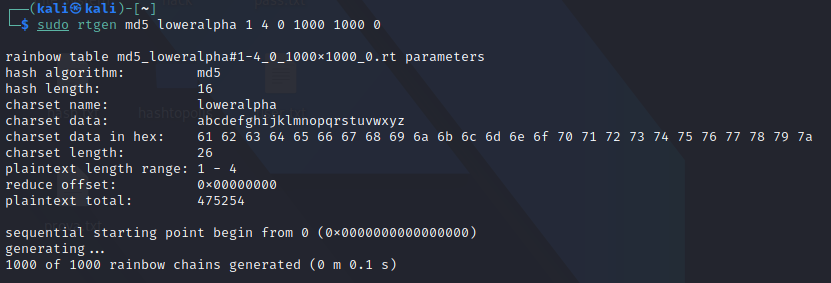
\includegraphics[width=120mm]{Immagini/1/r_1.png}
    \caption{RainbowCrack esempio generazione tabelle}
\end{figure}

Una volta generata la tabella, per utilizzarla dobbiamo prima caricarla, eseguendo il comando : 

\begin{lstlisting}[caption={RainbowCrack caricamento tabelle}, style=javaScriptCode]
    root@kali:~# sudo rtsort .
    \end{lstlisting}

Dopo aver caricato la tabella possiamo passare ad eseguire l'attacco, per eseguire l'attacco possiamo passare direttamente un hash ho passargli un file contenente gli hash da attaccare.

\begin{lstlisting}[caption={Esempio RainbowCrack command attack}, style=javaScriptCode]
    root@kali:~# sudo rcrack -h hash_da_attaccare
    root@kali:~# sudo rcrack -l path_file_da_attaccare
    \end{lstlisting}
\newpage
Ecco un esempio di un attacco :

\begin{figure}[h!]
    \centering
    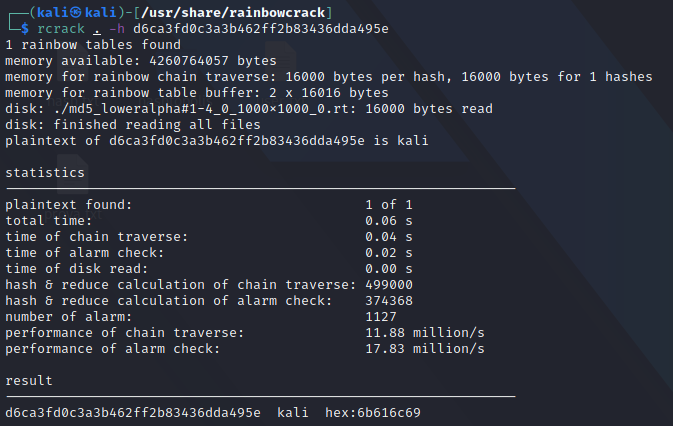
\includegraphics[width=100mm]{Immagini/1/r_2.png}
    \caption{Esempio RainbowCrack attack}
\end{figure}

Per evitare di cadere vittime di un attacco Rainbow Table, oltre a seguire tutte le buone pratiche durante la creazione di una password, questo tipo di attacchi possono essere facilmente prevenuti utilizzando la tecnica del Salt da parte dello sviluppatore del sistema IT in questione. 

Salt è un bit casuale di dati che viene passato nella funzione hash insieme al testo in chiaro. Ciò garantisce che ogni password abbia un hash generato univoco, rendendo impossibile eseguire questo tipo di attacco.

\section{Rule Attack}
L'attacco basato su regole\cite{Rule_based} è come un linguaggio di programmazione progettato per la generazione di password candidate. Ha funzioni per modificare, tagliare o estendere le parole e ha operatori condizionali per saltarne alcune. Ciò lo rende l'attacco più flessibile, accurato ed efficiente.
Questo tipo di attacco è applicabile nella maggioranza dei strumenti utilizzati per il Brute Force, gli esempi che andremo a vedere sono svolti utilizzando \textbf{Hashcat}, qui le regole vengono scritte in un file di configurazione, che successivamente verrà utilizzato in un comando per applicare le modifiche.

\begin{lstlisting}[caption={Utilizzo di regole su Hashcat }, style=javaScriptCode]
    root@kali:~# hashcat -r file_rules --stdout file_password
    \end{lstlisting}

La prima cosa che ci viene in mente è: quali sono le regole perché dovremmo usare Rule Attack per craccare l'hash. Quindi, prima di tutto, consideriamo il seguente scenario. Si ha un elenco di password di base contenente le seguenti parole :

\begin{lstlisting}[caption={Esempio rule attack wordlist}, style=javaScriptCode]
password
mysecret
qwerty
\end{lstlisting}
Se volessi provare le password aggiungendo il pattern "123" alla fine, dovremmo inserire all'interno del file delle regole il seguente comando "\textbf{\$1\$2\$3}", il comando \textbf{\&}, ci indica che deve essere applicato il carattere successivo alla fine di ogni parola contenuta nella wordlist.

La lista diventerà:
\begin{lstlisting}[caption={Risultato wordlist aggiunto il pattern "123"}, style=javaScriptCode]
password
password123
mysecret
mysecret123
qwerty
qwerty123
\end{lstlisting}

Se si vuole mettere in maiuscolo anche la prima lettera delle parole originali, dobbiamo inserire all'interno del file delle regole il comando "\textbf{c}", ora diventerà:
\begin{lstlisting}[caption={Esempio rule attack wordlist}, style=javaScriptCode]
password
password123
Password
mysecret
mysecret123
Mysecret
qwerty
qwerty123
Qwerty
\end{lstlisting}

Questo ci permette quindi di rendere più versatile il nostro attacco, andando a prendere un dizionario che abbiamo a disposizione e modificandolo in base alle nostre necessità.

Esistono molte altre regole che si possono applicare per cambiare la forma delle password, eccone alcuni :

\begin{table}[htbp]
    \begin{center}
    \begin{tabular}{|p{1.5cm}|l|p{4,3cm}|l|l|l|}
    \hline
    \textbf{Nome} & \textbf{Comando} & \textbf{Descrizione} & \textbf{Es} & \textbf{Input} & \textbf{Output} \\
    \hline
    Niente & : & non fa nulla & : & p@ssW0rd & p@ssW0rd\\
    \hline
    Minuscolo & io & Tutte le lettere minuscole	 & io & p@ssW0rd & p@ssw0rd	 \\
    \hline
    Maiuscolo & tu & Tutte le lettere maiuscole & tu & p@ssW0rd & P@SSW0RD\\
    \hline
    Inverti & C & Minuscolo prima lettera,& C & p@ssW0rd & p@SSW0RD \\
    maiuscolo&  &  maiuscolo il resto &  &  &  \\
    \hline
    Inverti m/M & t & Inverte m/M di tutti i caratteri nella parola. & t & p@ssW0rd & P@SSw0RD\\
    \hline
    Inverti m/M in N& TN & Invert m/M del carattere nella posizione N & T3 & p@ssW0rd & p@sSW0rd\\
    \hline
    Inversione & r & Invertire l'intera parola & r & p@ssW0rd & dr0Wss@p\\
    \hline
    Duplicare & d & Duplica parola intera & d & p@ssW0rd & p@ssW0rdp@ssW0rd\\
    \hline
    Riflettere & f & Parola duplicata e invertita & f & p@ssW0rd & p@ssW0rddr0Wss@p \\
    \hline
    Gira a sinistra & \{ & Ruota la parola a sinistra. & \{ & p@ssW0rd & @ssW0rdp\\
    \hline
    Gira a destra & \} & Ruota la parola a destra & \} & p@ssW0rd & dp@ssW0r \\
    \hline
    Aggiungi carattere & \textasciicircum X & Anteponi il carattere X in primo piano & \textasciicircum 1 & p@ssW0rd & 1p@ssW0rd\\
    \hline
    \end{tabular}
    \end{center}
    \caption{Esempio regole hashcat}
    \label{tab:browser}
    \end{table}

\section{Mask Attack}
Gli attacchi con maschera \cite{Mask_attack} sono simili agli attacchi di forza bruta, negli attacchi di forza bruta, vengono provati tutte le possibili combinazioni esistenti. Gli attacchi con maschera sono più specifici poiché il set di caratteri che provi viene ridotto in base alle informazioni che si conosce.

Ad esempio, se si sa che l'ultimo carattere di una password è un numero, puoi configurare la maschera per provare solo i numeri alla fine. Usando i tradizionali attacchi di forza bruta, saresti comunque costretto a provare tutte le combinazioni che non sono numeri.

Ad esempio, se prendiamo la seguente password: \textbf{Maschera101}

Ha una lunghezza di 7 caratteri e per ognuno può essere maiuscolo (26 potenziali caratteri), minuscolo (26 potenziali caratteri), un simbolo (33 potenziali caratteri) o un numero (10 potenziali caratteri), noi dovrei provare un numero totale di \({95}^{7}\) (69.833.728.698.375) combinazioni.

Supponiamo ora di sapere che gli ultimi tre caratteri sono numeri. Ciò ridurrebbe drasticamente il potenziale spazio delle chiavi poiché non sarebbe necessario provare password con lettere o simboli negli ultimi tre spazi.

Vediamo un esempio pratico di un Mask attack. Sappiamo che la password del hash che abbiamo recuperato è lunga 6 e composta da tutte lettere minuscole, il comando che andremo ad eseguire (con Hashcat) è il seguente :

\begin{lstlisting}[caption={Esempio rule attack wordlist}, style=javaScriptCode]
    root@kali:~# hashcat -m 0 -a 3 2906de51196732ba0b97eb5360c1baeb ?l?l?l?l?l?l
    \end{lstlisting}

Ed otterremo il seguente risultato :

\begin{figure}[h!]
    \centering
    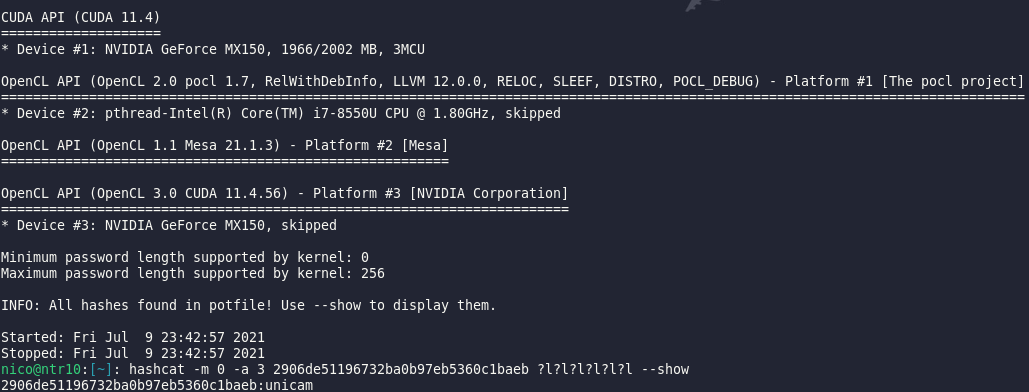
\includegraphics[width=\linewidth]{Immagini/1/mask.png}
    \caption{Esempio Mask Attack con Hashcat}
\end{figure}

Ovviamente devi assicurarti che le tue informazioni sulla password siano corrette, altrimenti la tua maschera potrebbe non generare la password. Usando il mascheramento puoi anche creare maschere per sfruttare le abitudini delle password. Ad esempio, un'abitudine comune è che le password inizino con una maiuscola se ne è richiesta almeno una.

Un altro esempio in cui è possibile applicare il mascheramento è quando si conosce il pattern della password da attaccare. Molti router domestici hanno algoritmi di generazione di password predefiniti e le informazioni sulla creazione delle loro chiavi possono essere trovate online.

In questi tipi di attacco, come abbiamo potuto vedere nell'esempio precedente, dobbiamo passare la maschera secondo uno speciale codifica, questa è :

\begin{itemize}
    \item \textbf{?u} = lettera maiuscola
    \item \textbf{?l} = lettera minuscola
    \item \textbf{?d} = numero
    \item \textbf{?s} = carattere speciale
\end{itemize}

Questi vengono composti per creare la nostra maschera da utilizzare per la realizzazione delle password da testare nell'attacco.

Vediamo alcuni esempi di maschere che si possono creare :

\begin{table}[htbp]
    \begin{center}

    \begin{tabular}{|l|l|}
        \hline
        \textbf{Password} & \textbf{Maschera} \\
        \hline
        Unicam1336 & ?u?l?l?l?l?l?d?d?d?d \\
        \hline
        cAmErInO! & ?l?u?l?u?l?u?l?u?s \\
        \hline
        Laurea?20-21 & ?u?l?l?l?l?l?s?d?d?s?d?d \\
        \hline
    \end{tabular}
\end{center}
\caption{Esempio maschere per password}
\end{table}